
\renewcommand{\EntradaBibtex}{AppSegmentaCromosomas_SistemasInteligentes_UPV_2023}


\begin{frame}{\citetitle{\EntradaBibtex} \footnotemark[1] (1)}
\begin{block}{Motivación} 
Desarrollar aplicación móvil para que el Citogenetista localice los cromosomas en imágenes de estudios de citogenética y genere el Cariograma
\end{block} 
\begin{itemize}
\item El usario selecciona una carpeta con imágenes de cromosomas y la imagen de trabajo. 
\item Se incluyen funciones de paneo y acercamiento/alejamiento
\item Con el dedo hacer trazos sobre los cromosomas (definir el esqueleto). Personalizar el grosor y el color del trazo.
\item Una vez finalizado el trazo pregunta el número de cromosoma recién seleccionado (23 pares de cromosomas)
\item Al seleccionar todos los cromosomas, generar el Cariograma
\end{itemize}
\footnotetext[1]{\fullcite{\EntradaBibtex}}
\end{frame}

\begin{frame}{\citetitle{\EntradaBibtex} (2)}

\begin{center}
	\begin{tabular}{ccccc}
		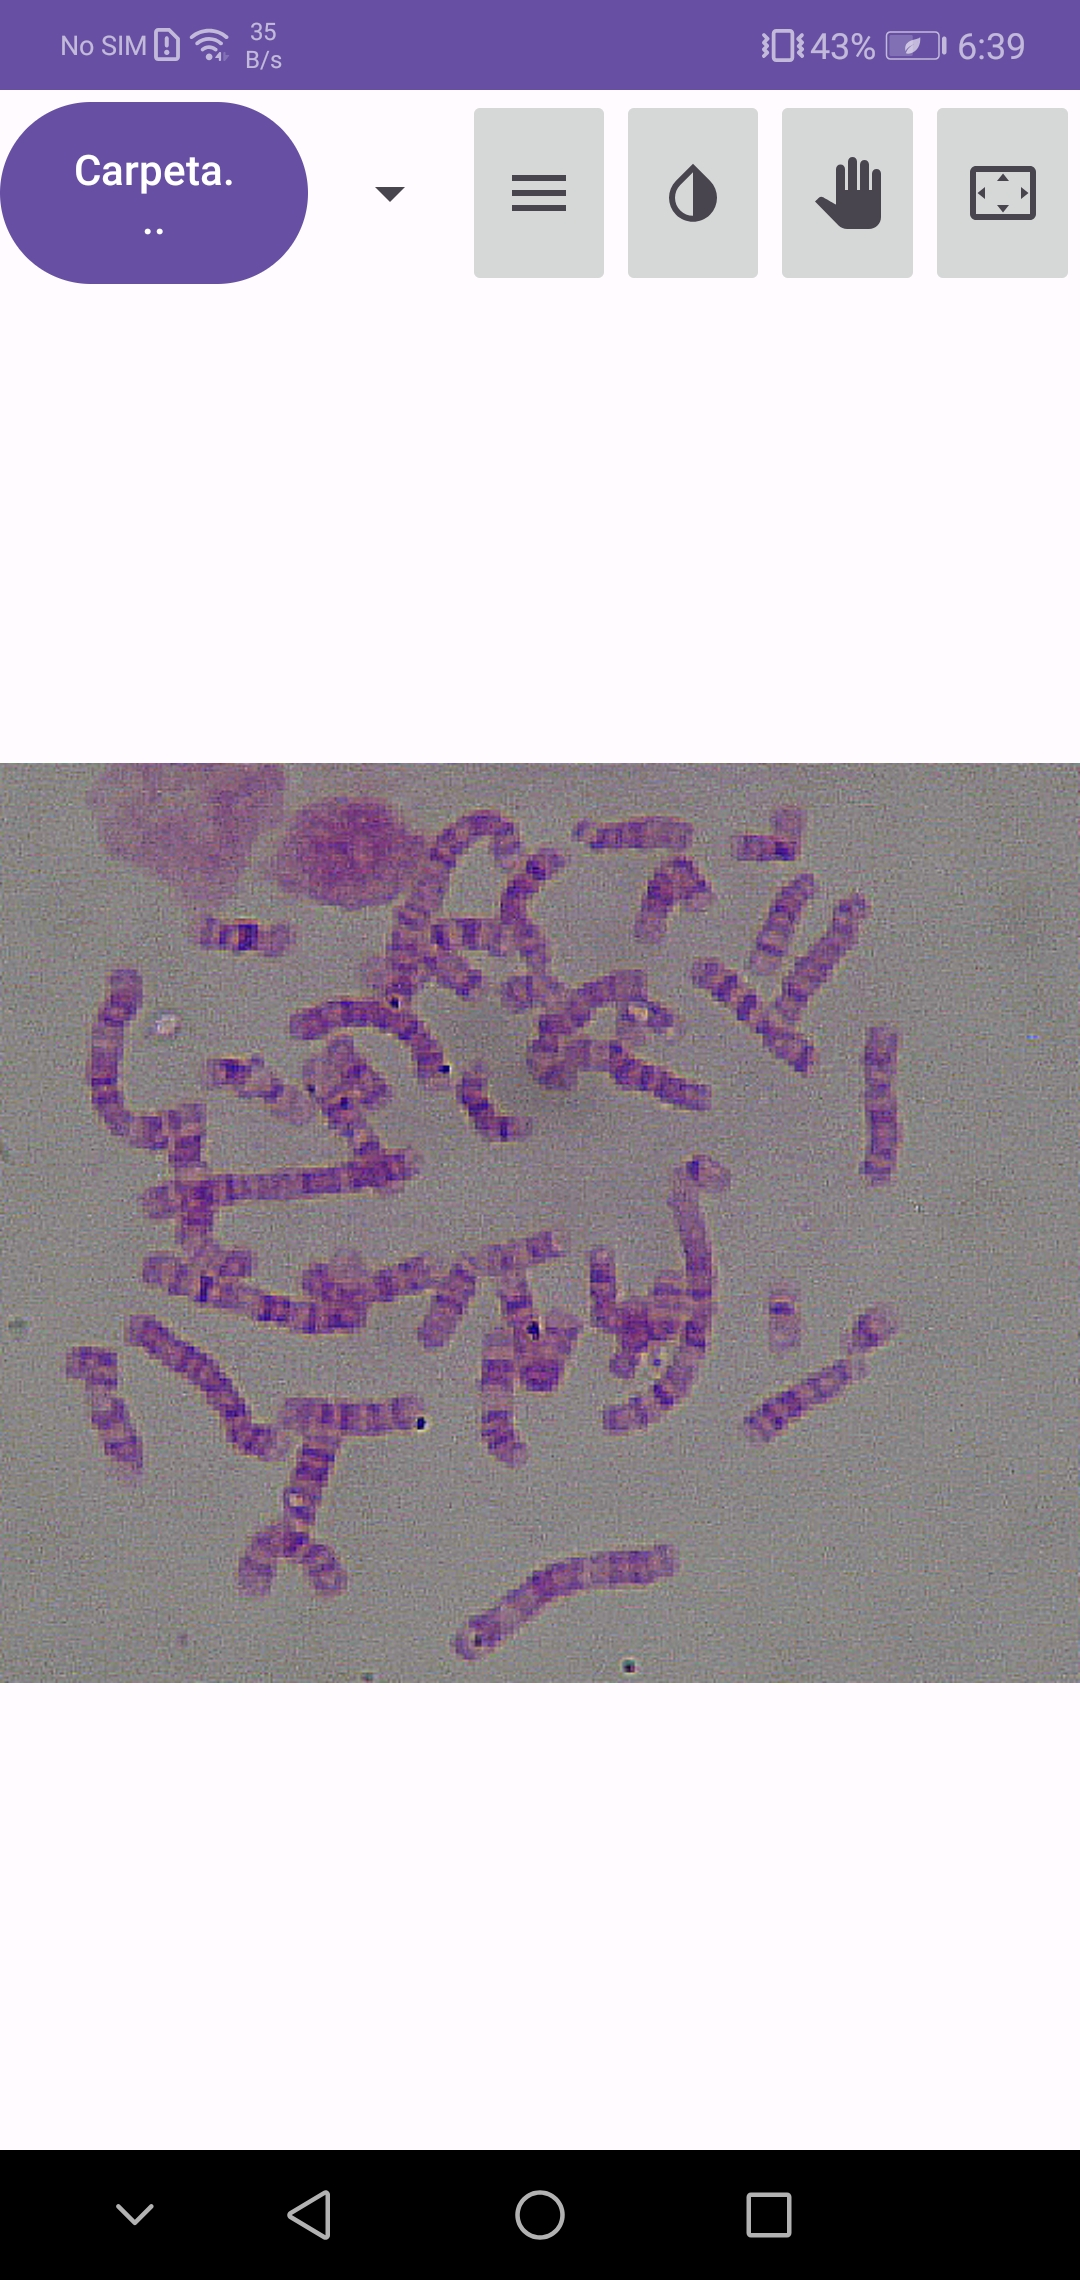
\includegraphics[width=0.18\linewidth,height=4.85cm]{2023_AppSegmentaCromosomas/figs/vistadeimagen.jpg}  &
		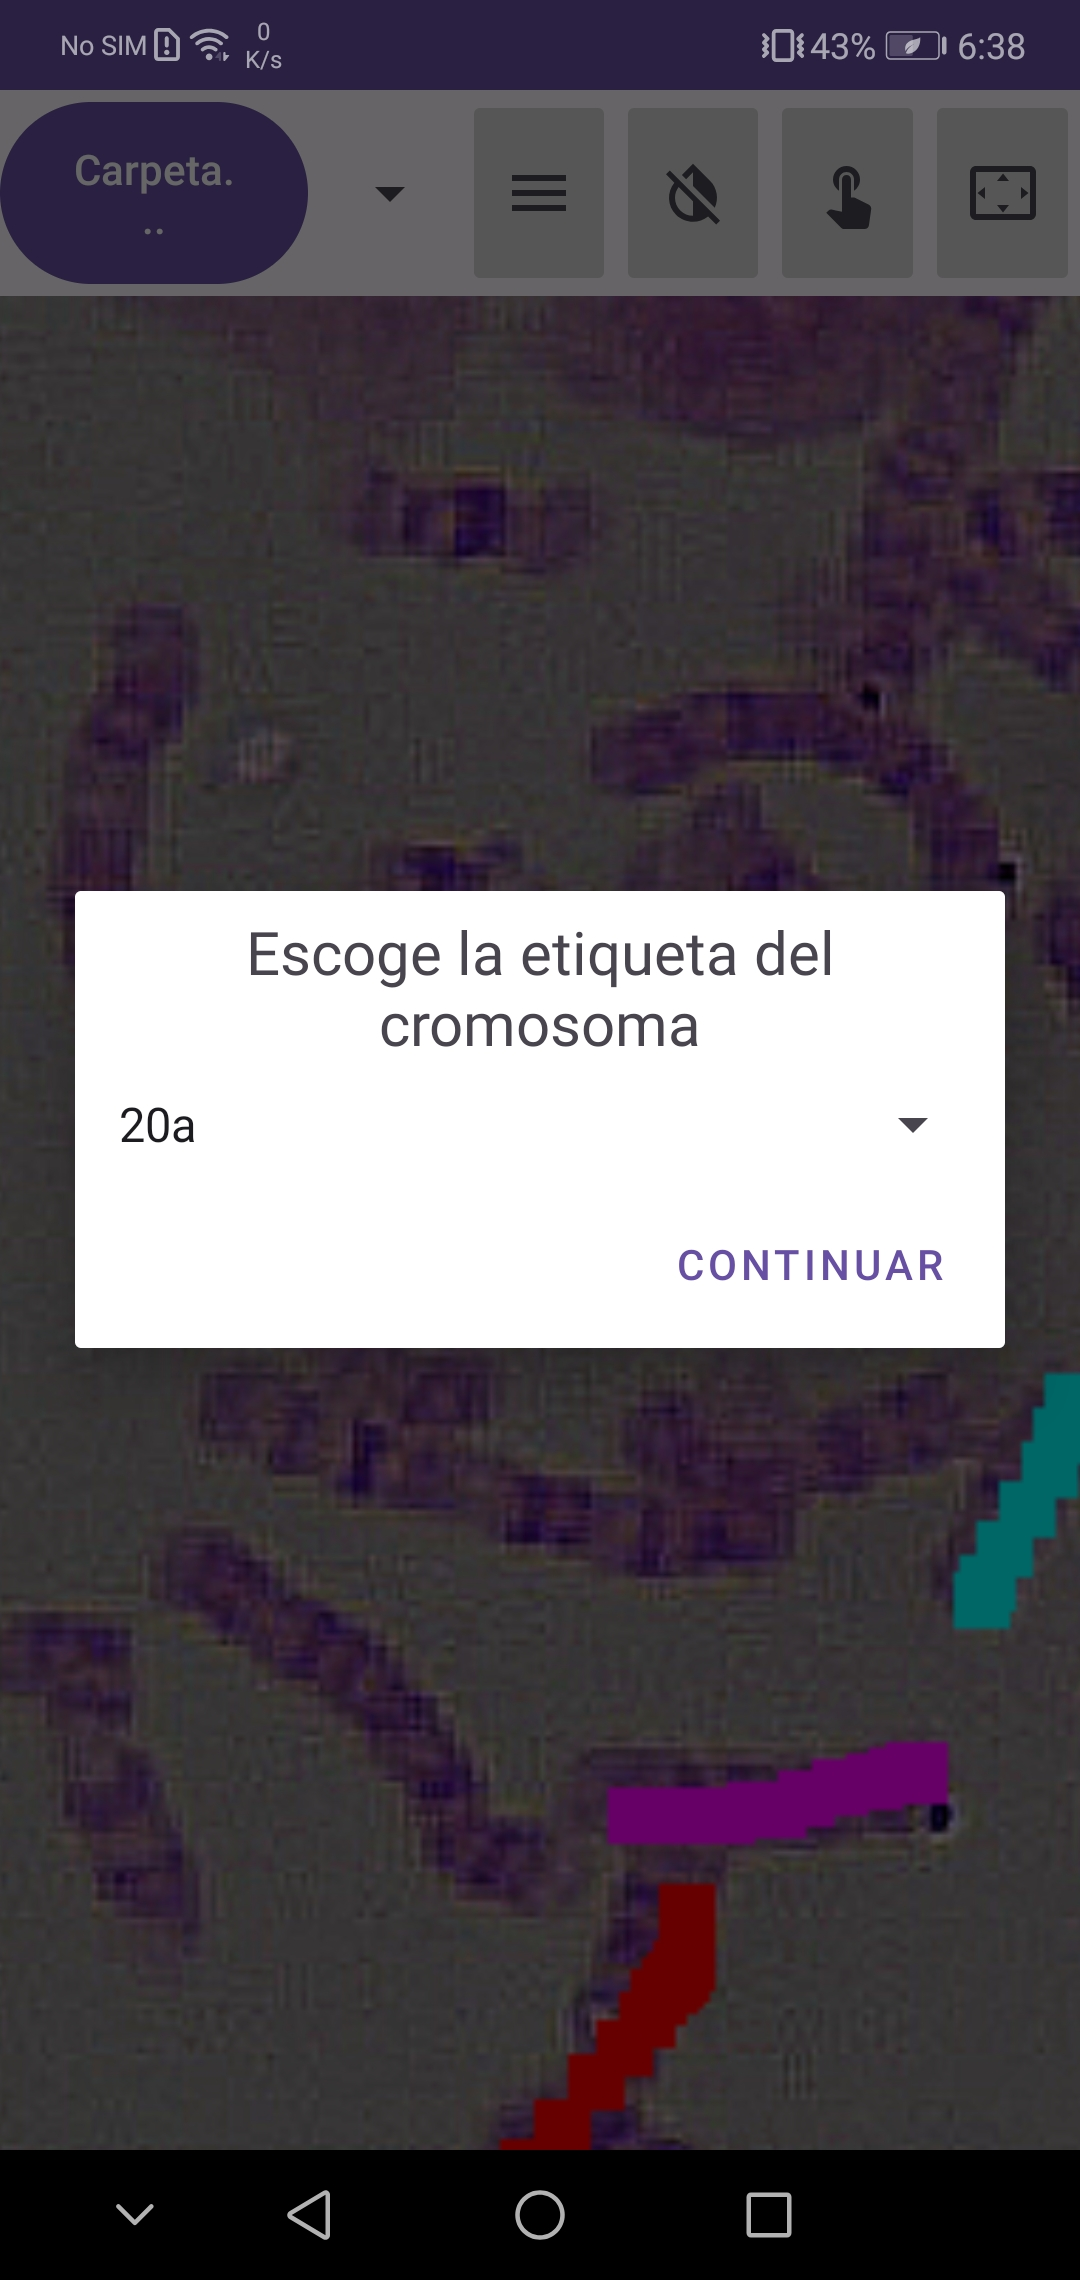
\includegraphics[width=0.18\linewidth,height=4.85cm]{2023_AppSegmentaCromosomas/figs/trazado.jpg} &		
		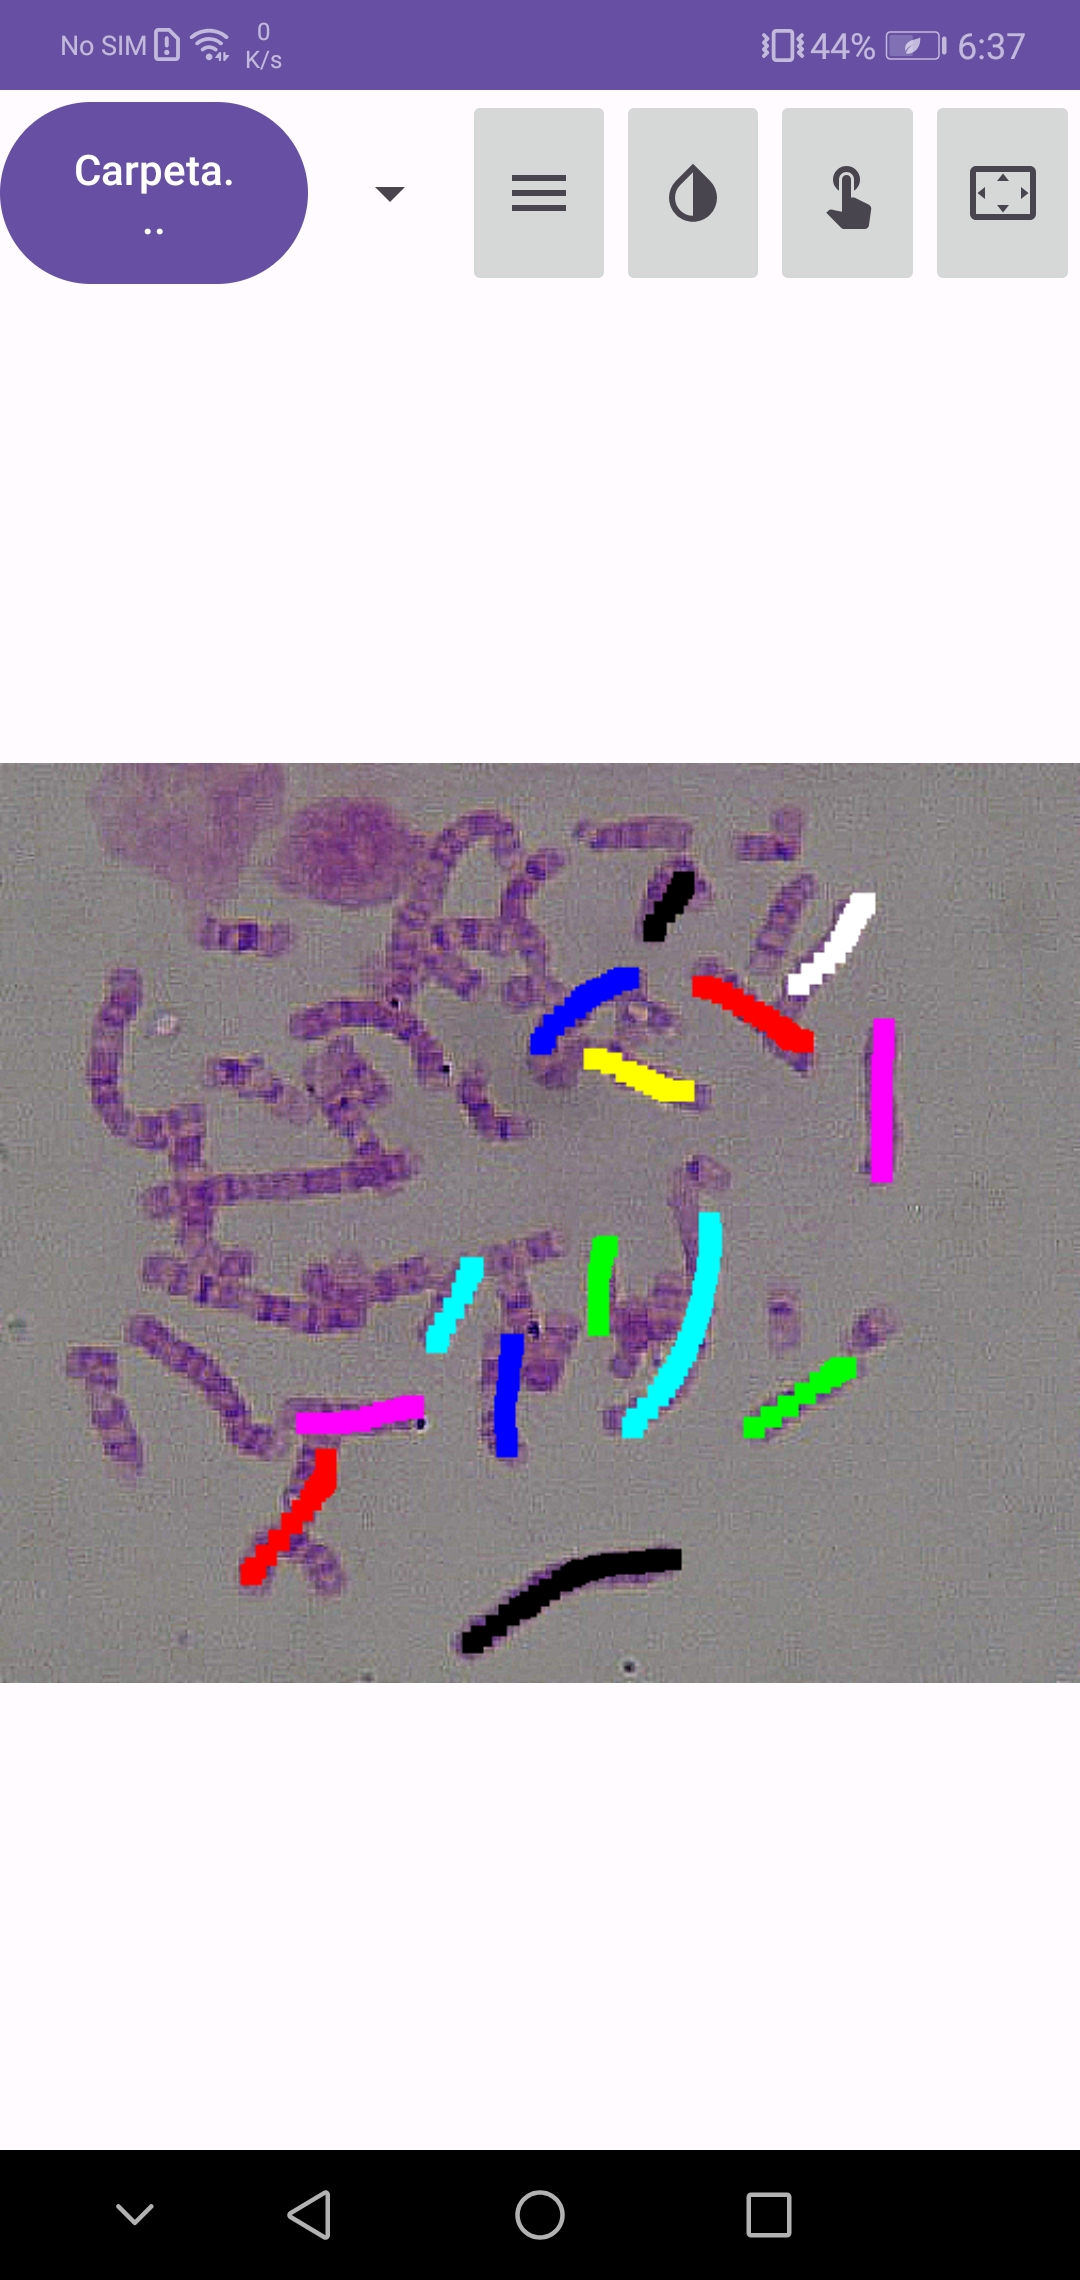
\includegraphics[width=0.18\linewidth,height=4.85cm]{2023_AppSegmentaCromosomas/figs/ediciondetrazo.jpg} &
		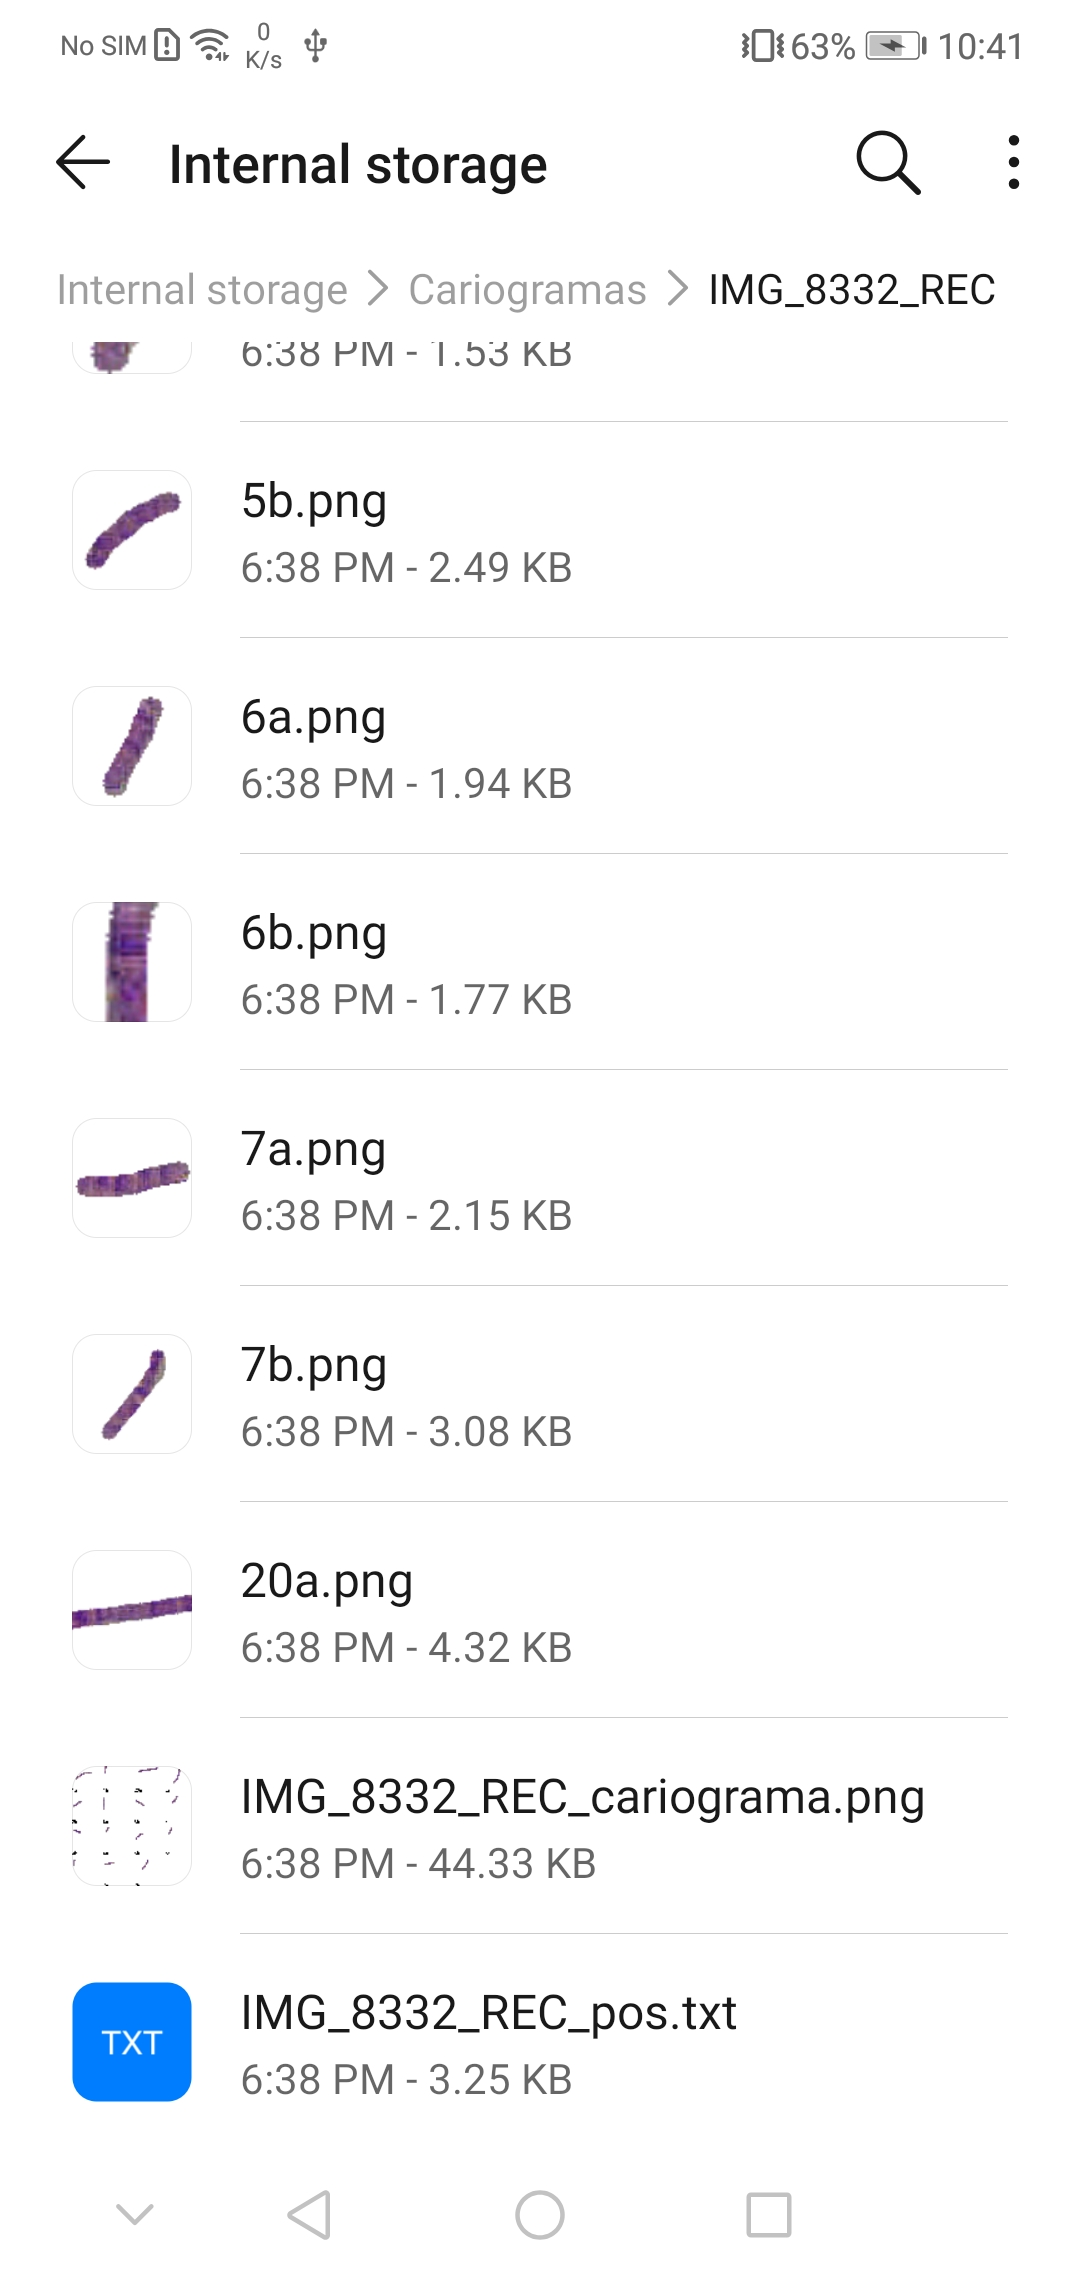
\includegraphics[width=0.18\linewidth,height=4.85cm]{2023_AppSegmentaCromosomas/figs/archivosdescargados.jpg} &
		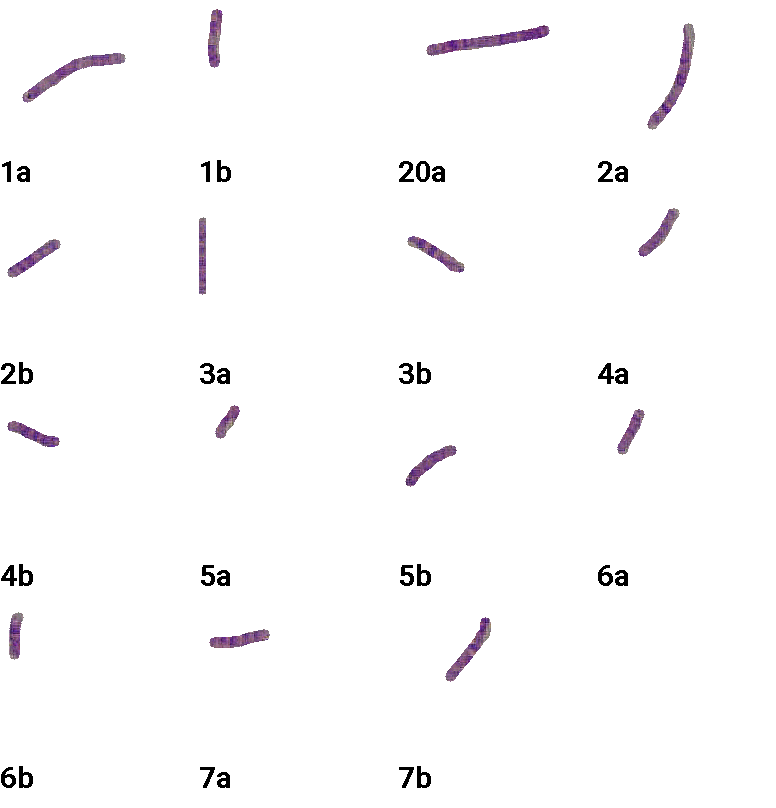
\includegraphics[width=0.18\linewidth,height=4.85cm]{2023_AppSegmentaCromosomas/figs/cariograma.png} \\
	\end{tabular}
\end{center}

\end{frame}


\begin{frame}{\citetitle{\EntradaBibtex} (3)}

\begin{center}
		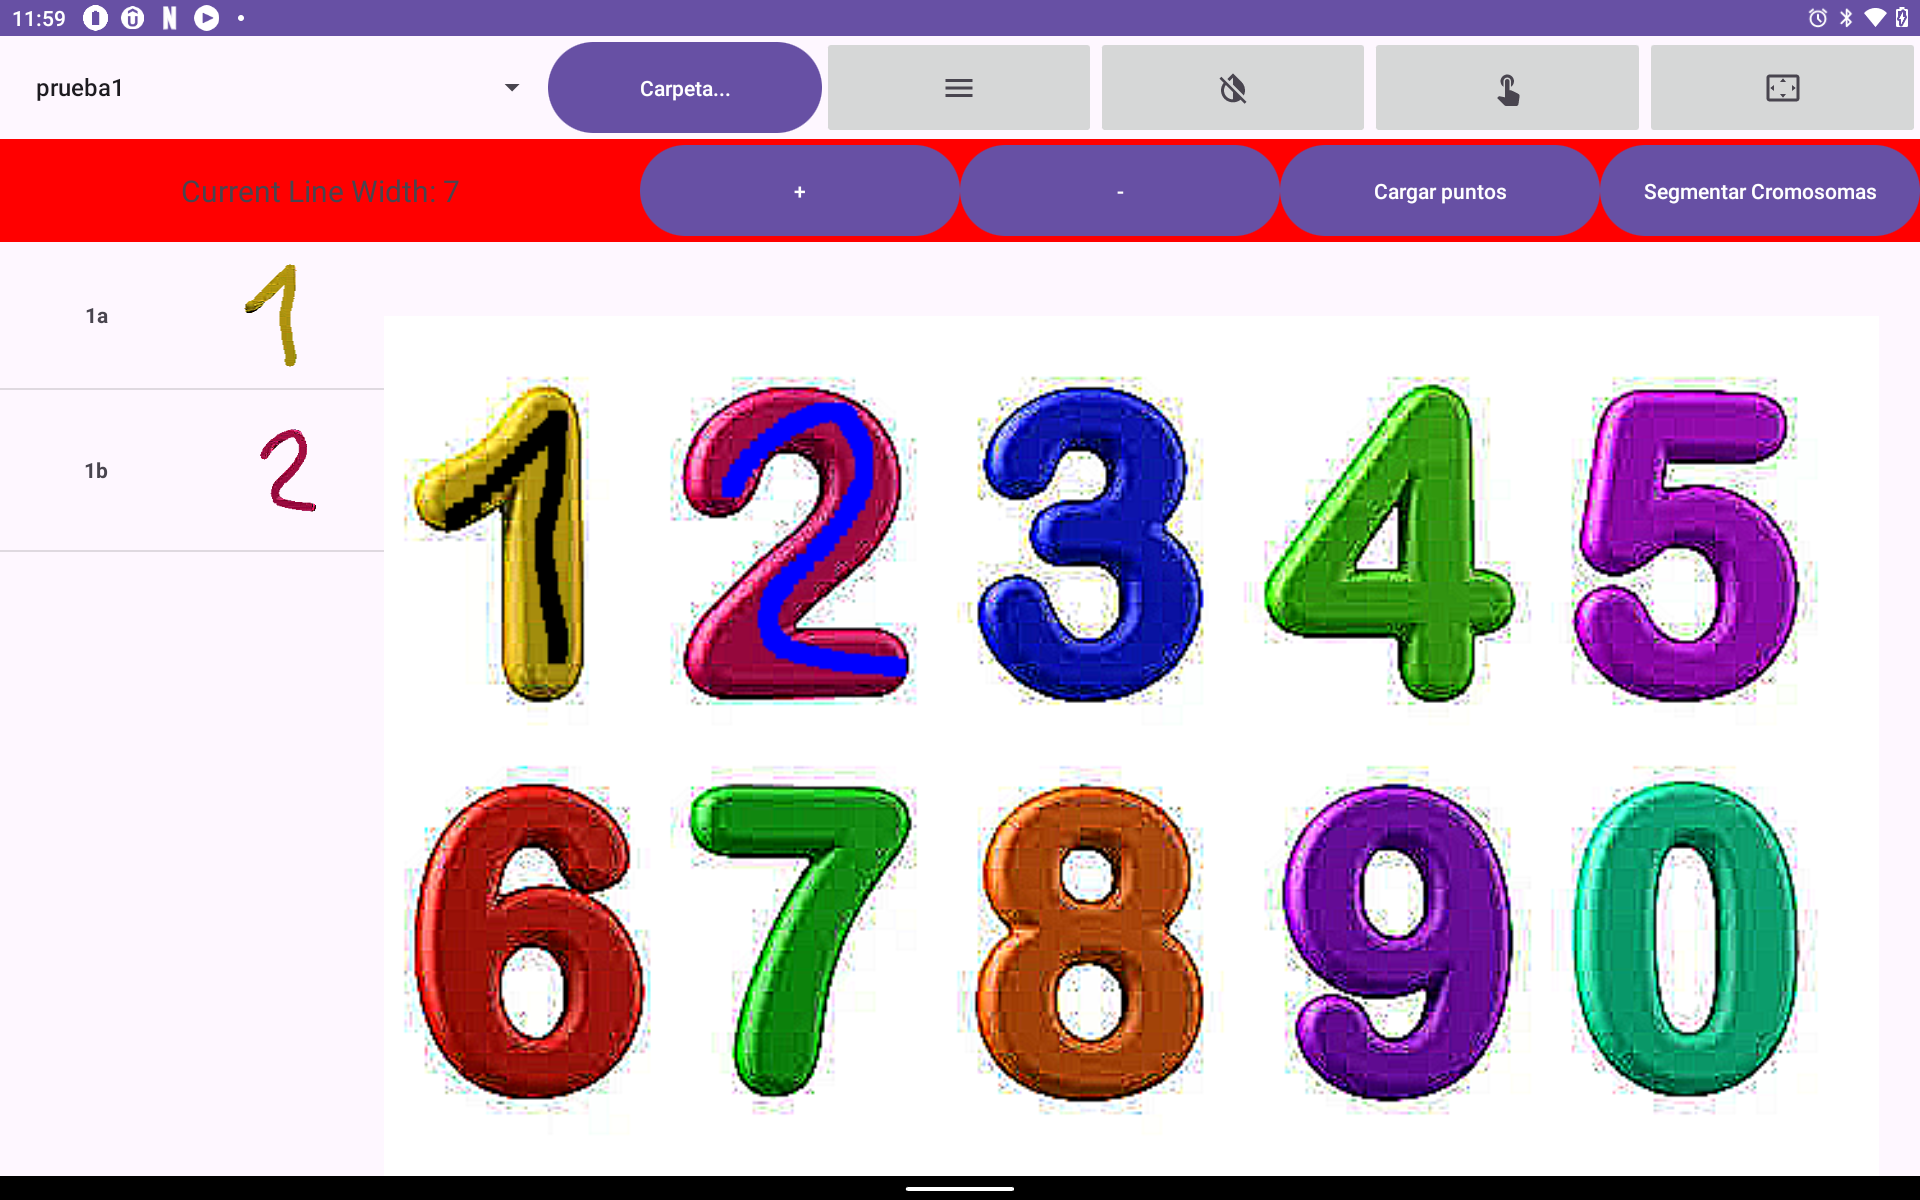
\includegraphics[width=0.70\linewidth]{2023_AppSegmentaCromosomas/figs/AppCromosomasTablet.png}  
\end{center}

\end{frame}


%


